\section{Auswertung}
\label{sec:Auswertung}
Ein typisches Signalbild der Messung ist in \ref{fig:Signal} dargestellt. Die beiden
Resonanzstellen sind rechts von dem Nullpeak zu finden. Bevor den Resonanzstellen einem
der beiden Rubidium Isotope zugeordnet werden kann, wird der erste Peak rechts von dem Nullpeak
dem \textit{Isotop 1} und der zweite dem  \textit{Isotop 2} zugeordnet.
\begin{figure}
  \centering
  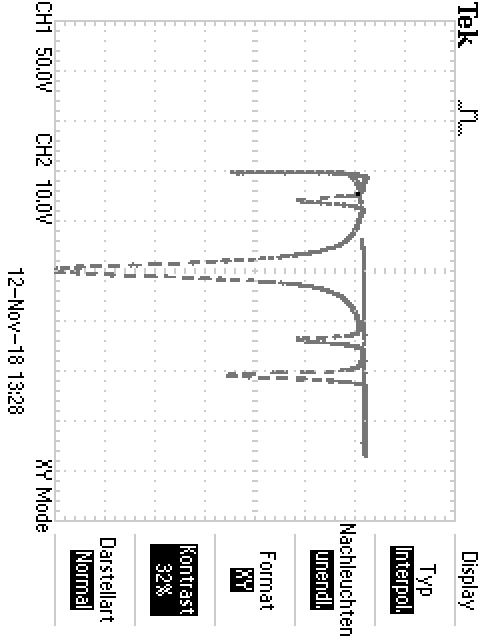
\includegraphics[angle=90]{pics/TEK0000.JPG}
  \caption{Typisches Signalbild auf dem Oszilloskop. Es sind der Nullpeak (mittig) und
           die Resonanzstellen der beiden Isotope zu sehen (rechts).}
  \label{fig:Signal}
\end{figure}
Die Breite des Nullpeaks ist Abhängig von der vertikalen Komponente des Erdmagnetfeldes.
Um den Einfluss der vertikalen Komponente des Erdmagnetfeldes so gering wie möglich zu halten
und damit den Peak zu verschmälern wird der Versuchsaufbau in Nord-Süd-Richtung gedreht und ein
Feld in vertikale Richtung angelegt.
An die vertikal ausgerichtete Helmhotzspule wird ein Strom $I= 0,231$ V angelegt. Damit
ergibt sich mit der magnetischen Feldkonstante $\mu_{0}$, der Windungszahl $N$ der Spule,
dem Radius $R$, dem Strom $I$ und der Helmhotzgleichung
\begin{equation}
  B=\mu_{0}\frac{8 N }{\sqrt{125} R}I
\end{equation} eine Feldstärke von $B_{\text{vertikal}}=35,40 \mu$ T.
Der Literaturwert der Vertikalkomponente liegt bei (?? Litwert 44 microT ??).
\subsection{Bestimmung der Landéschen $\text{g}_{\text{F}}$ Faktoren}
Zwischen der Magnetfeldstärke $B$ und der Frequenz $f$ an den Resonanzstellen besteht der Zusammenhang
\begin{equation}
  B=\frac{\text{h}f}{\mu_{\text{B}} \text{g}_{\text{F}}} .
\end{equation}
Dieser Zusammenhang ist in \ref{fig:BFelder} aufgeführt. Es wurde eine Gerade der
Form $y=m\cdot x+b$ an die Messwerte der beiden Isotope gefittet. Die Fitparameter sind dabei
\begin{align*}
  m_1&=(1,04 \pm 0,05)\,\frac{\mu\text{T}}{\text{kHz}} \\
  b_1&=(-120,7 \pm 0,3)\,\mu\text{T}\\
  m_2&=(1,4 \pm 0,1)\,\frac{\mu\text{T}}{\text{kHz}} \\
  b_2&=(-238,5 \pm 0,6)\,\mu\text{T}
\end{align*}
\begin{figure}
  \centering
  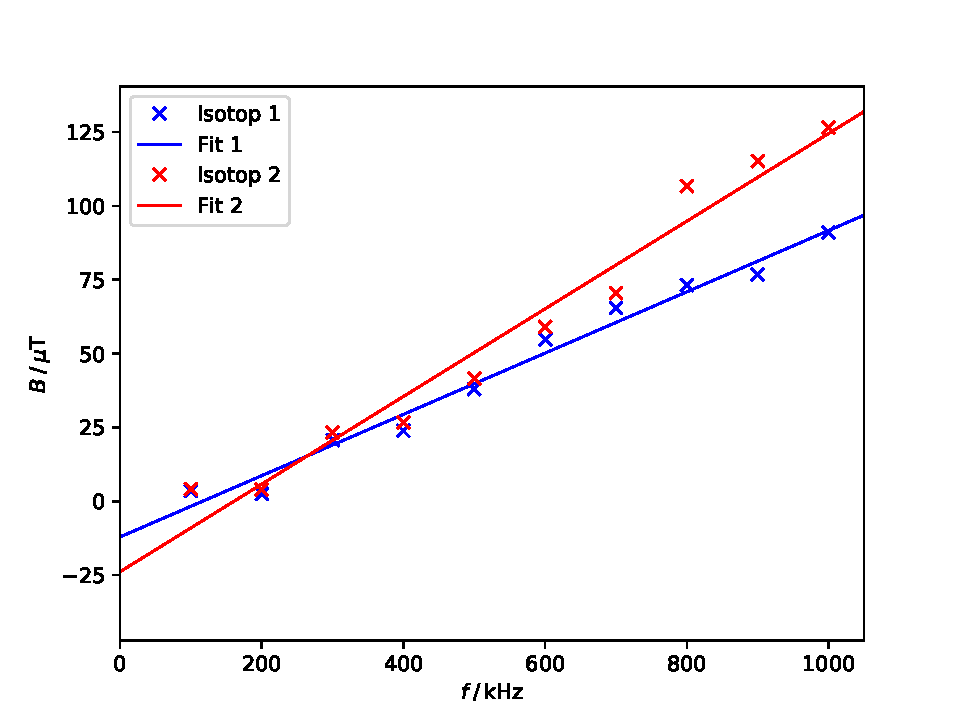
\includegraphics{plots/BFelder.pdf}
  \caption{}
  \label{fig:BFelder}
\end{figure}
Daraus lassen sich die Landéschen $\text{g}_{\text{F}}$ Faktoren mit
\begin{equation}
  \text{g}_{\text{F}}=\frac{\text{h}}{\mu_{\text{B}}} \frac{f}{B}
\end{equation}
bestimmen, wobei das Verhältnis von Magnetfeld uns Frequenz durch die
Steigung $m=B/f$ ausgedrückt werden kann.\\
Damit lassen sich die Landéschen $\text{g}_{\text{F}}$ Faktoren zu:
\begin{align*}
  \text{g}_{\text{F,1}}=0,069 \pm 0,003
  \text{g}_{\text{F,2}}= 0,049 \pm 0,003
\end{align*}
berechnen.\\
Das Verhältnis der beiden 
% \begin{figure}
%   \centering
%   \includegraphics{plots/plot.pdf}
%   \caption{Plot.}
%   \label{fig:plot}
% \end{figure}



% \begin{table}
%    % Notation :  {% nicht entfernen ist sehr wichtig sonst Fehler !!
% \parbox{0.48\textwidth}{% %Ermöglicht zwei Tabellen neben einander
%   \centering
%   \sisetup{round-mode = places , round-precision = 0,scientific-notation=fixed, fixed-exponent = 0}
%          %rundet Werte aus Stelle, Stelle = ,  macht einen bestimmten festen exponenten
%   \resizebox{\textwidth}{!}{%  % skaliert zu große Tabellen
%   \begin{tabular}{S@{${}\pm{}$} S} % fügt plus minus Fehler Schreibweise hinzu
%     \toprule
%      $\text{e}_b / \si{\milli\meter}$ &
%      $\text{d}_b /\si{\milli\meter} $ & $\text{f}_b / \si{\milli\meter} $\\
%     \midrule
%     \bottomrule
%   \end{tabular}
%   % }
%   \caption{Tabellenunterschrift}
%   \label{tab:tab}
% }
% % \end{table}
% % \begin{table}
% \parbox{0.48\textwidth}{%
%   \centering
%   \sisetup{round-mode = places , round-precision = 0,scientific-notation=fixed, fixed-exponent = 0}
%   % \resizebox{\textwidth}{!}{%
%   \begin{tabular}{S@{${}\pm{}$} S}
%     \toprule
%      $\text{e}_b / \si{\milli\meter}$ &
%      $\text{d}_b /\si{\milli\meter} $ & $\text{f}_b / \si{\milli\meter} $\\
%     \midrule
%     \bottomrule
%   \end{tabular}
%   % }
%   \caption{Tabellenunterschrift}
%   \label{tab:tab}
% }
% \end{table}
